\section{Implementation}\label{sec:implement}

%-----------------------------------------------------------------------------
\subsection{Omni XMP Compiler Framework}
%-----------------------------------------------------------------------------

The CAF translator was added into the Omni XMP compiler as shown in Figure~\ref{fig:translator}.
The Omni XMP compiler is a source-to-source translator that converts XMP programs 
into the base language (Fortran or C).  The component `coarray translator' is 
located in front of the XMP translator to solve coarray features previously. 
The output of the decompiler is a standard Fortran/C program that may include 
calls to the XMP runtime library.

The following procedures are generated in advance or in the coarray translator
to initialize static coarray variables prior to the execution of the user program:
\begin{itemize}
\item
The built-in main program calls subroutine {\tt xmpf\_traverse\_init},
the entry procedure of initialization subroutines, before executing the
user main program.
\item
Subroutine {\tt xmpf\_traverse\_init} is generated by the coarray translator 
to call initialization subroutines corresponding to all user-defined procedures.
\item
Each initialization subroutine {\tt xmpf\_init\_{\it foo}} is generated from 
user-defined procedure {\it foo} by the coarray translator. 
It initializes all static coarrays declared in {\it foo}.
\end{itemize}

\begin{figure}[tbh]
 \begin{center}
  % trimはleft bottom right topの順
  %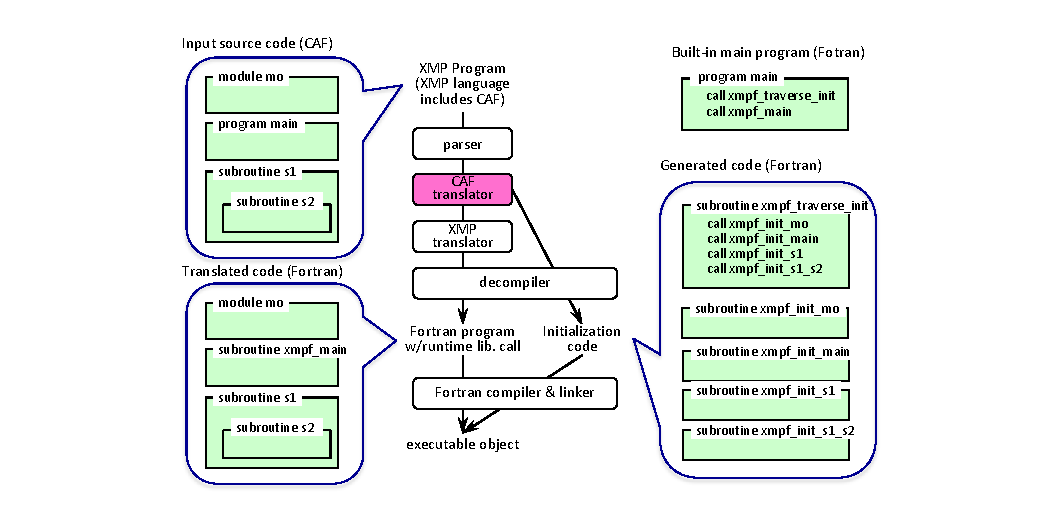
\includegraphics[scale=0.55,trim=6cm 0cm 4cm 6cm,clip]{figs/translator-tmp.pdf}
  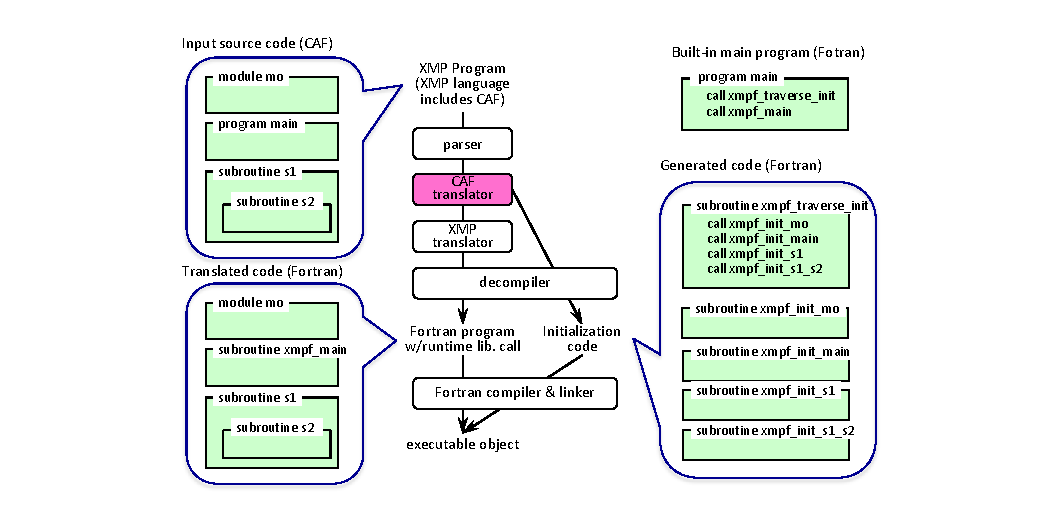
\includegraphics[trim=30mm 0mm 20mm 7mm, scale=1.0]{figs/translator-tmp.pdf}
  \caption{XMP compiler and an example of coarray program compilation}
  \label{fig:translator}
  %-- 修正すべき箇所
  CAF translator $\rightarrow$ coarray translator
 \end{center}
\end{figure}


%-----------------------------------------------------------------------------
\subsection{Allocation and Registration}
%-----------------------------------------------------------------------------

To be accessed using the underlying communication library,
the allocated coarray data must be registered to the library.
The registration contains all actions to allow the data to be accessed 
from the other nodes, including pin-down memory, acquirement of the global address,
and sharing information among all nodes.

%===========================================================
\subsubsection{Three methods of memory management}
%===========================================================

The coarray translator and the runtime library implements three methods of
memory management.
\begin{itemize}
\item
The {\bf Runtime Sharing (RS) Method} allocates and registers a large memory 
for all static and dynamic coarrays at the initialization phase.
The registered memory is shared by all static and allocatable coarrays. 

\item
The {\bf Runtime Allocation (RA) Method} allocates and registers a large memory
for all static coarrays at the initialization phase.
And it allocates and registers each allocatable coarray at runtime.

\item
The {\bf Compiler Allocation (CA) Method} allocates all coarray objects by 
the Fortran system (at compile time or at runtime) and the address is 
passed to the runtime library to be registered.
\end{itemize}

For the RS and RA methods, 
because the allocated memory address is determined in the runtime library, 
the object code must accept the address allocated 
inside the runtime system as an address of a regal Fortran variable.
To make this connection, it was necessary to use the Cray pointer, which is not 
in the Fortran standard.
In the case of the CA method, the runtime library accepts the address allocated
in the Fortran system, and registers to the communication library.

%
% 3 methodsの比較表を載せるならここか
%


%===========================================================
\subsubsection{Initial Allocation for Static Coarrays}
%===========================================================

Static coarrays are allocated and registered in the initialization subroutines 
{\tt xmpf\_init\_{\it foo}}. 

On the RS and RA methods,
static coarrays are initialized before the execution of the user program,
as follows.
\begin{itemize}
\item
In the first pass, all sizes of static (non-allocatable) coarrays are summed.
The size of each static coarray is evaluated form the lower and upper bounds
specified in the dimension declaration statement of each coarray.
The lower and upper bound expressions, possibly including binary and unary
operations, reference to name of constants, and basic intrinsic functions 
such as min/max and sum, are evaluated by constant folding techniques.
Since the size of the structure that contains allocatable or pointer 
components differs depending on for the target compiler, the coarray translator
get the necessary parameters to calculate the size of structures at the build time.
\item
Then, the total size of static coarrays is allocated and the address
and the size is registered to the underlying communication library.
\item
In the second pass, the addresses of the all coarrays are calculated to share
the registered data.
Due to the language specification, sizes of the same coarray are the same 
among all images (nodes). So the offset from the base address of the registered 
data for each coarray can be the same among all images.
\end{itemize}
%
In the RS method, allocatable coarrays are also shared the registered memory. 
The total size of the memory to be registered
should be specified with an environment variable by the user.
While in the RA method, the total size is fully calculated by the runtime 
library and no information is required to the user because allocatable coarrays
will be dynamically allocated on the other memories.

On the CA method,
the Fortran processor allocates each coarray and then the runtime library
registers the address.
Each static coarray is converted into a common (external) variable to share 
between the user-defined procedure (say {\it foo}) and its initialization
procedure ({\tt xmpf\_init\_{\it foo}}). The data is statically allocated
by the Fortran system similarly to the usual common variable.
the address is registered in the initialization procedure via the runtime
library.


%===========================================================
\subsubsection{Runtime Allocation for Allocatable Coarrays}
%===========================================================

For the RS method, the runtime library has a memory management system for
cutting out and retrieving memory for each allocation and deallocation of 
coarrays.

Figure~\ref{fig:register-RA-CA} illustrates the memory allocation and registration
for allocatable coarrays on the RA and CA methods. 

\begin{figure}
 \begin{center}
  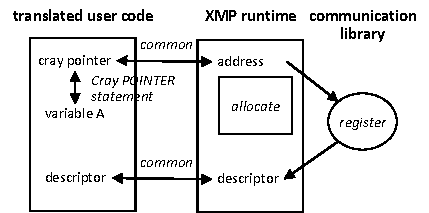
\includegraphics[scale=0.9, trim=0mm 0mm 0mm 0mm, clip]{figs/register-RA-tmp.pdf}\\
The runtime allocates and registers coarrays and passes the address to the user code.
 \end{center}
 \begin{center}
(a) RA method
 \end{center}
 \begin{center}
  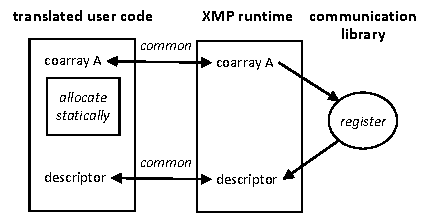
\includegraphics[scale=0.9, trim=0mm 0mm 0mm 0mm, clip]{figs/register-CA-tmp.pdf}\\
The user code allocates coarrays and causes the runtime to register with the address.
 \end{center}
 \begin{center}
(b) CA method
 \end{center}
 \caption{Memory allocation for coarrays in RA and CA methods}
 \label{fig:register-RA-CA}
\end{figure}

These methods are properly used by the underlying communication library.
%
On GASNet, only the RS method is adopted because its allocation function
can be used only once in the program.
%
On MPI-3, the CA method is not suitable because frequent 
allocation and deallocation of coarrays cause expensive creation and freeing 
MPI windows.
%
Over FJ-RDMA, the RS method has no advantage over the other methods.
Since the allocated address is used for registration to FJ-RDMA, 
no advantage was found for managing memory outside of the Fortran system. 
The unusual connection through the Cray pointer causes the degrade of 
the Fortran compiler optimization.


%-----------------------------------------------------------------------------
\subsection{PUT/GET Communication}\label{sec:putget}
%-----------------------------------------------------------------------------

To avoid disturbing the execution on the remote image, PUT and GET communications
are implemented always using Remote Direct Memory Access (RDMA) provided by 
the communication library (except coarrays with pointer/allocatable structure components). 
In contrast, local data access is selective between using Direct Memory Access (DMA) or
using a local buffer. For the buffer scheme, one of four algorithms will be chosen.


%===========================================================
\subsubsection{Determining the possibility of DMA}\label{sec:opt-dma}
%===========================================================

coarray変数は割付け時にregistrationすることでRDMAアクセス
が可能になる。一方で、PUTのsourceまたはGETのtargetとなるローカル側
データは、registrationされていなければどのDMAの対象にならないので、
あらかじめregistrationされたバッファを介して通信することになる。
しかし、ローカルデータもregistrationされたcoarrayであることは比較的
多く、その場合にはDMAできる。
ローカルデータが仮引数の場合、それがregistratedかどうか
は実行時にしか分からないので、runtimeによる判定が望ましい。

runtime libraryでは、ローカルデータがregistrationされているか否かをbinary treeで
判定する仕組みを持っている。これは以下のように実現されている。
\begin{itemize}
\item
When a chunk of coarray data is registered to the communication library, 
runtime library adds the set of the local address and the size into a sorted 
table called SortedChunkTable. The sort key is the local address.
\item
When a chunk of coarray data is deregistered from the communication library, 
runtime library deletes the record in SortedChunkTable.
\item
When a PUT or GET runtime library is called corresponding to a referrence/definition
to a coindexed object/variable, the local address is searched in SortedChunkTable
with binary search. The local data is already registrated if 
$addr_i \leq addr < addr_i + size_i$ for any $i$,
where $addr$ is the said local address and $add_i$ and $size_i$ are the
$i$-th address and size in SortedChunkTable, respectively.
\end{itemize}

データ量が大きい場合、この判定のコストは相対的に
十分小さいので、まずこの判定を行い、可能ならDMA-RDMA通信を行っている。
データ量が小さいときには、この判定の時間よりバッファリングする時間の方が短くなる
ため、バッファリングを選ぶ。


%===========================================================
\subsubsection{Buffering Communication Methods}
%===========================================================

For the buffer scheme, one of four algorithms will be chosen 
depending on three parameters, the size of the local buffer $B$ and the 
local and remote contiguous lengths $N_L$ and $N_R$.
$B$ should be large enough to ignore communication latency overhead and we use
about 400 kilo-bites in default. Unlike the case of MPI message passing,
coarray PUT/GET communication requires only one local buffer for any numbers of
other images.
$N_L$ and $N_R$ can be evaluated at runtime. The Fortran syntax guarantees 
that $N_L$ is a multiple of $N_R$ or $N_R$ is a multiple of $N_L$.
An algorithm to get the contiguous length is shown in the paper~\cite{pgas15}.

\tab{putget} summarizes our algorithm for PUT/GET communication for five cases.
The unit size is the chunk length of the PUT/GET communication.
Case~0 shows the algorithm using RDMA-DMA PUT/GET communication and Cases~1 through~4
shows the algorithms using RDMA and local-buffering. 
Due to its strict condition, the DMA scheme is rarely used.
And it is not always faster than the buffering scheme cases~2 and~3 because of the 
difference of the unit sizes. The merit of cases~2 and~3 is that the unit size 
is extended to a multiple of $N_L$ by gathering number of short contiguous data in the buffer,
or by scattering from the buffer into number of short contiguous data.

\begin{table}[tbh]
 \caption{Summary of the PUT/GET algorithm related to $N_L$, $N_R$ and $B$}
 \label{tab:putget}
 \begin{flushleft}
  \begin{tabular}{|@{~}c@{~}|c||@{~}c@{~}|@{~}c@{~}|}
\hline
scheme &
case &
condition &
unit size \\
\hline
\hline
DMA &
&
Local data is registered. &
$\min(N_L, N_R)$ \\
\hline
buffering &
1 & 
$N_R \leq B,~ N_R \leq N_L$ &
$N_R$ \\
\cline{2-4}
&
2 &
$N_L < N_R \leq B$ &
$N_R$ \\
\cline{2-4}
&
3 &
$N_L < B < N_R$ &
multiple of $N_L$ ($\leq B$) \\
\cline{2-4}
&
4 &
$B < N_R,~ B \leq N_L$ &
$B$ (or less than $B$ at last) \\
\hline
  \end{tabular}
 \end{flushleft}
 \begin{flushleft}
  \begin{tabular}{|@{~}c@{~}|c||@{~~}l@{~~}|@{~~}l@{~~}|}
\hline
scheme &
case &
PUT action for each unit &
GET action for each unit \\
\hline
\hline
DMA &
&
put once &
get once \\
\hline
buffering &
1 &
buffer once and put once &
get once and unbuffer once \\
\cline{2-4}
&
2 &
buffer for each $N_L$, and put once &
get once, and unbuffer for each $N_L$ \\
\cline{2-4}
&
3 &
buffer for each $N_L$, and put once &
get once, and unbuffer for each $N_L$ \\
\cline{2-4}
&
4 &
buffer once and put once &
get once and unbuffer once \\
\hline
  \end{tabular}
 \end{flushleft}
\end{table}


%===========================================================
\subsubsection{Non-blocking PUT communication}
%===========================================================

PUT通信をできる限りnon-blockingとし、そして、その完了待ちを可能なら次のimage control statementまで遅延したい。
\fig{block-ex}に示したような、同じsegment内で同じリモートデータへ書いて読むような
ケースは大変まれで、殆どの場合には次のimage control statementまで遅延できる。
添字式やイメージ番号が定数でないことが多いので、コンパイル時の判定では遅い方に倒れてしまう。
まれなケースだけを軽いコストで正しく除外できる実行時判定が望まれる。

現在の実装では、実行時の環境変数によってblockingとnon-blocking通信を選択する。
以下の条件に該当する場合には、低速となるblockingを選択しなければならない。
 リモートのcoarrayデータを更新した後で、同じセグメントの中で、同じデータを参照している。
ほとんどの場合には該当しないことを利用者が分かるので、non-blockingのオプションを
選択することを期待する。


%===========================================================
\subsubsection{Optimization of GET communication}\label{sec:opt-get}
%===========================================================

A referrence to an array coindexed object is converted to a call of a runtime library 
function that returns a Fortran array value. For example, array assignment statement:
\begin{verbatim}
  b(j1:j2) = a(i1:i2)[k] 
\end{verbatim}
is converted to:
\begin{verbatim}
  b(j1:j2) = xmpf_coarray_get_generic(dp_a,k,a(i1:i2)) 
\end{verbatim}
by the coarray translator, where {\tt dp\_a} is the descriptor of coarray {\tt a}.
The result value of the function is one-dimensional array whose size 
is $({\tt i2} - {\tt i1} + 1)$.
The issue is that it tends to cause many data copies in some library layers.
As a contermeasure, we optimized specfic but common case by the translator.
If a coindexed object is only the right-hand side of an array assignment statement,
the entire assignment statement can be converted into one library call.
The example above satisfies the condition, so it can be converted again as follows:
\begin{verbatim}
  call xmpf_coarray_getsub_generic(dp_a,k,a(i1:i2),b(j1:j2)) 
\end{verbatim}
In this runtime library subroutine, the variable {\tt b(j1:j2)} is expected to be 
the local target of GET communication instead of the local buffer that would be
generated by the Fortran runtime.


%-----------------------------------------------------------------------------
\subsection{Runtime Libraries}\label{sec:runtime}
%-----------------------------------------------------------------------------

The layer of the runtime libraries are shown in \fig{layer}.
One of three communication libraries is selected 
at the build time of the Omni compiler.
The coarray runtime consists of layered three libraries.
\begin{itemize}
\item
The {\bf lower-level runtime library (LRL)} abstracts the difference between 
the communication libraries except the memory management of coarray data.
\item
The {\bf upper-level runtime library (URL)} solves each coarray features 
in the coarray program.
\item
The {\bf Fortran wrapper} mediates the arguments and the result value 
of the translated user program (written in Fortran) and URL (written in C).
\end{itemize}


\begin{figure}[tbh]
  \begin{center}
    % trimはleft bottom right topの順
    %\mbox{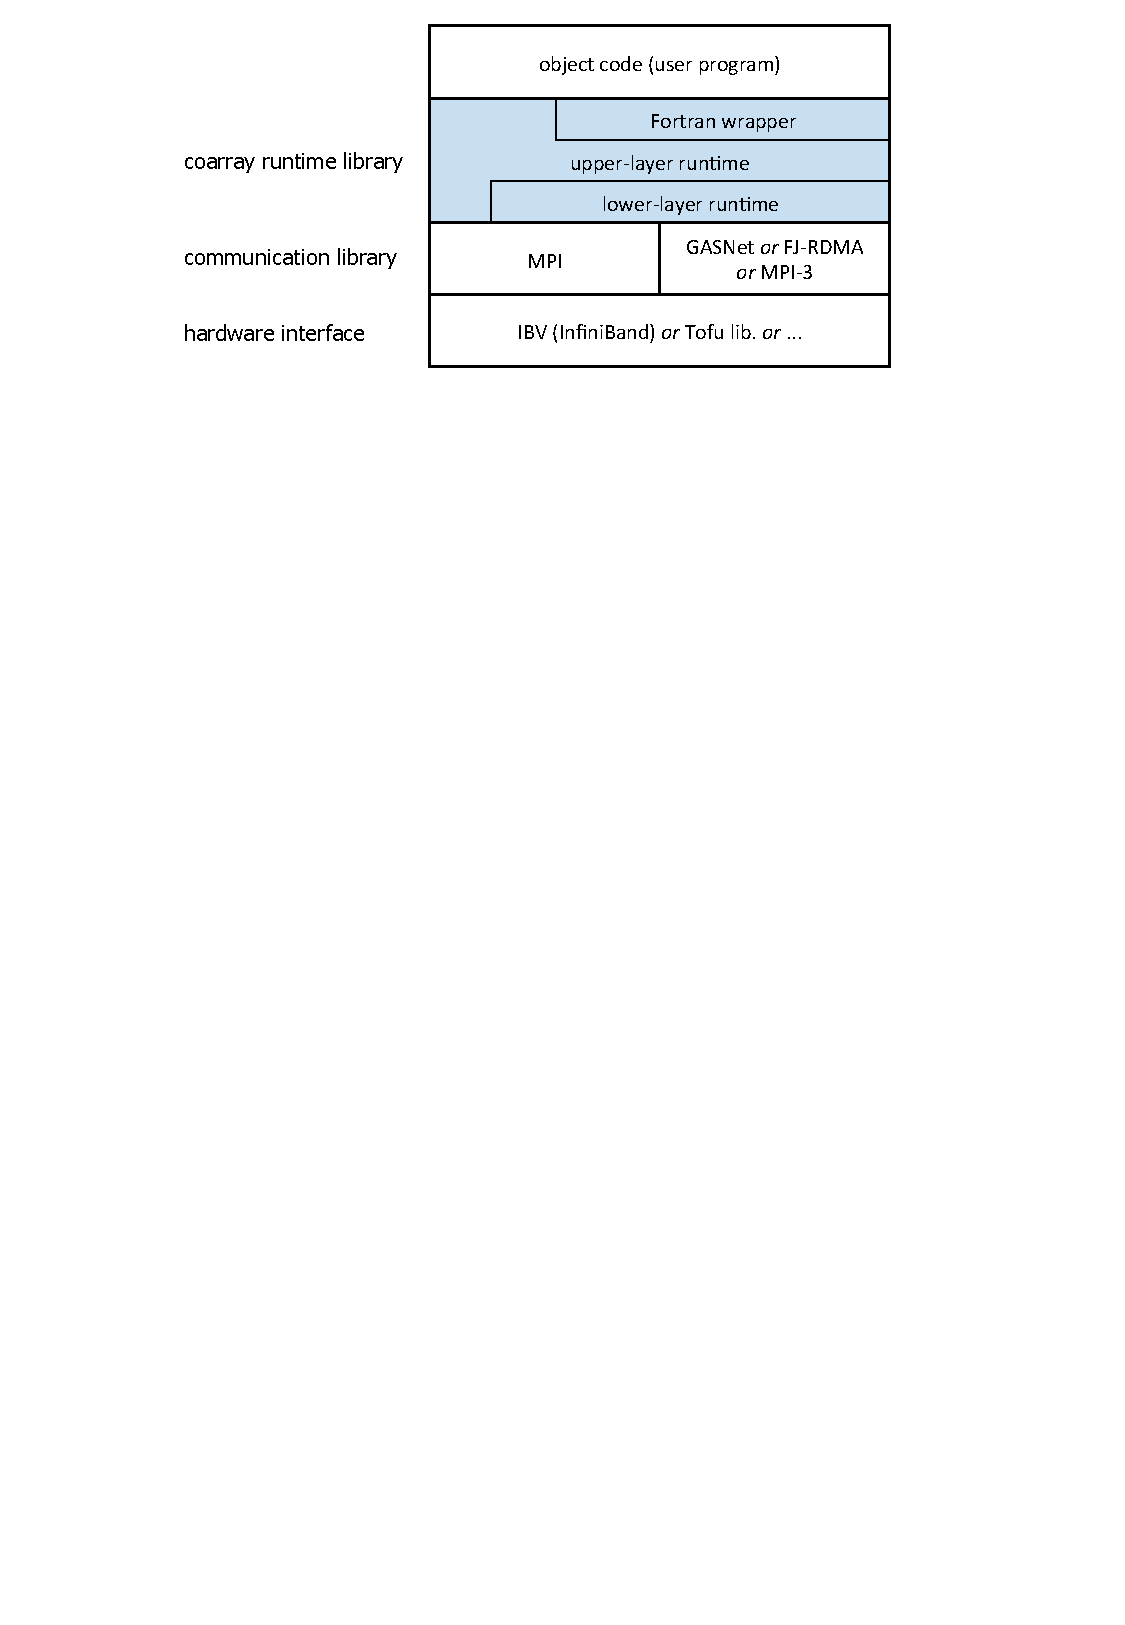
\includegraphics[trim=42mm 210mm 47mm 0mm, scale=0.7,clip]{figs/softstack-r2.pdf}}
    \mbox{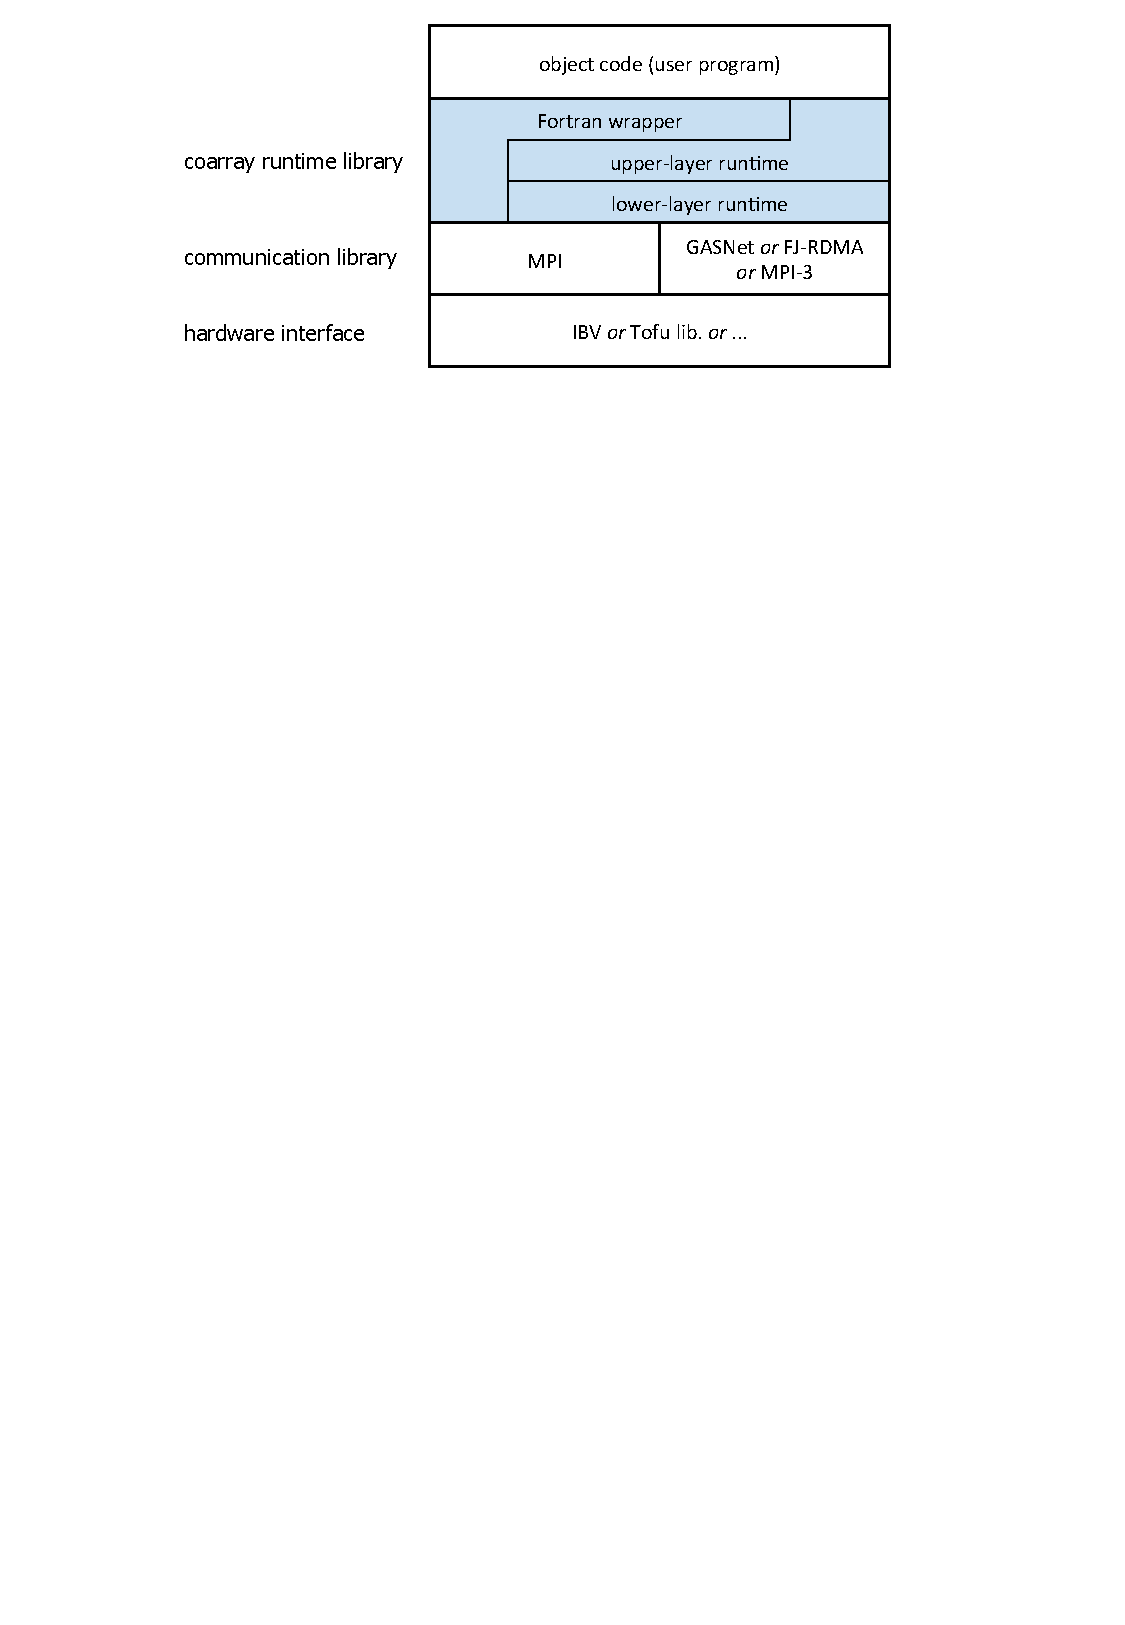
\includegraphics[trim=27mm 208mm 29mm 0mm, scale=0.7,clip]{figs/softstack-r4.pdf}}
    \caption{Software stack for coarray features}\label{fig:layer}
  \end{center}
\end{figure}


%===========================================================
\subsubsection{Underlying Communication libraries}
%===========================================================

MPI-3 can be selected for all platform on which MPI-3 is implemented. Coarrays are 
registered and deregistered at the start and end point of the MPI window. 
Coarrays are performed one-sided communication by {\tt MPI\_Put} and {\tt MPI\_Get},
and synchronized by {\tt MPI\_Win\_fence}. 
Implementation on MPI incurs certain costs for dynamic allocation of coarrays and 
waiting for communication completion.

GASNet can be selected for more advanced implementation over InfiniBand. 
Since allocation and registration of are inseparable and can be done only once 
on GASNet, the implementation allocates and registers a pool of memory
whose size should be large enough to contain all static and allocatable coarrays.
The XMP runtime should allocate and deallocate coarrays not using the Fortran 
library but using the memory manager made for the pool.

FJ-RDMA can be selected for the implementation over Tofu interconnect of 
the K computer and Fujitsu PRIMEHPC FX series supercomputers. 
Basically, each coarray is allocated by the Fortran library and registered 
the address with the FJ-RDMA interface {\tt FJMPI\_Rdma\_reg\_mem}. 
And it is deregistered with {\tt FJMPI\_Rdma\_dereg\_mem} before deallocated 
(freed) by the Fortran library. 
One-sided communication is performed with {\tt FJMPI\_Rdma\_put} and 
{\tt FJMPI\_Rdma\_get}.
%, which include confirmation of communication completion. <-- 本当? いつも?


%===========================================================
\subsubsection{Fortran wrapper}
%===========================================================

While the coarray runtime is written in C, coarray features are 
based on array notations specified in Fortran~90 or later.
The Fortran wrapper is a part of the coarray runtime and mediates
Fortran and C argument interfaces.

For example, suppose {\\tt a} is a two-dimensional array coarray of 
16-byte complex type. The value of a coindexed object:
\begin{center}\tt
a(1:10,2:19)[{\it k}]
\end{center}
should be a two-dimensional array shaped {\tt [} 10, 18 {\tt ]}. 
The coarray translator converts it to a wrapper function call:
\begin{center}\tt
xmpf\_coarray\_get\_generic({\it desc\_}a, {\it k}, a(1:10,2:19))
\end{center}
where {\tt{\it desc\_}a} is the descriptor of coarray {\tt a}.
Note that the generic function name is used in the output of the coarray
translator. The corresponding specific name is selected in the 
following Fortran compiler as shown below:
\begin{center}\tt
xmpf\_coarray\_get2d\_z16({\it desc\_}a, {\it k}, a(1:10,2:19))
\end{center}
where {\tt xmpf\_coarray\_get2d\_z16} means the wrapper function
of GET communication for two-dimensional and 16-byte complex type.
The last argument is a mold expression to get the communication pattern 
and the shape of the result value.
At last, this function invokes the C-written runtime function:
\begin{center}\tt
xmpf\_coarray\_get\_array({\it desc\_}a,\,base,\,16,\,{\it k},\,dst,\,2,\,skip,\,extent)
\end{center}
where, 
%
{\tt base} is the address of {\tt a(1,2)} that is the base address of {\tt a(1:10,2:19)},
%
{\tt dst} is the result variable of 16-byte complex shaped {\tt [} 10, 18 {\tt ]}
in Fortran, or, the pointer to 16 $\times$ 10 $\times$ 80-byte memory in C, and
%
{\tt skip} and {\tt extent} are two-dimensional integer arrays to represent 
the pattern of the communication data.

As shown in this example,
the Fortran wrapper converts Fortran multi-dimensional array segments 
into a set of contiguous data sequences, which can be handled in the runtime
library written in C.
Conversely, it makes data returned from the runtime library an array, 
in the case of GET communication to an array coarray.
It also converts a C pointer to a Fortran pointer with the shape, using
the Cray pointer.

本実装では、Fortranの高級な仕様(配列記述や総称名手続き)を
runtime libraryインタフェースとした。
これにより、コンパイラが生成すべきオブジェクトインタフェースの数を
数十分の一に削減してデータの型と形状をruntimeに伝えることができる
ようになった。

For collective commnications, which are caused by intrinsic subroutines 
{\tt CO\_SUM}, {\tt CO\_MAX}, {\tt CO\_MIN} and {\tt CO\_BROADCAST}, 
the Fortran wrapper uses MPI library functions directly.
%
For one-sided and collective communications, it uses URL.


%Actually, the interface is used through the Fortran~90 generic interface
%to ease the code generation by the coarray translator.
%For example, let us convert an {\tt ALLOCATE} statement
%{\tt allocate (a(1:10,2:19))}, where {\tt a} is an allocatable coarray of 16-byte,
%using object-ULR interface {\tt XMPCO\_malloc\_coarray}.
%The translator may generate a call to the generic procedure \\
%{\tt xmpf_coarray_malloc_generic(descriptor_of_a, a, 


%===========================================================
\subsubsection{Upper-layer runtime library (URL)}
%===========================================================

The major role of URL is performing the algorithm shown in \Sec{putget}
for one-sided PUT/GET communications.
It uses LRL for blocking or non-blocking data transfer 
between pre-registered local and pre-registered remote data.

For atomic communications caused by intrinsic subroutines
{\tt ATOMIC\_DEFINE} and {\tt ATOMIC\_REF}, 
URL calls the corresponding function of LRL after address calculation.


%===========================================================
\subsubsection{Lower-layer runtime library (LRL)}
%===========================================================

LRL basicly abstracts the difference between the communication libraries.
The only exception is about allocation and registration of coarray data.
The object code should exclusively select one of the following set:

\begin{itemize}
\item
Functions to allocate and register a coarray data at the same time
and functions to deregister and free it at the same time.
The functions are supporsed to be used in the RS and RA methods and
suitable for GASNet.

\item
Functions to register an already-allocated coarray data 
and functions to deregister it.
The functions are supporsed to be used in the CA method and
not suitable for GASNet.
\end{itemize}

Other major LRL functions are shown bellow.
\begin{itemize}
\item
A set of functions to allocate and register a specified size of coarray,
and a set of functions to register an already-allocated coarray.
They are alternatively used in the RS and RA methods and in the CA method.
Corresponding to each, a set of functions to deregister and deallocate and
a set of functions to deregister are provided.

\item
A function for RDMA-DMA GET communication with specified-length contiguous
data, and the one of DMA-RDMA PUT communication.
They assume that both remote and local data are previously registered.
Blocking and non-blocking can be switched and the only way to wait for
the completion of the non-blocking communication is using the function
corresponding to {\tt SYNC MEMORY}.

\item
Functions corresponding to the {\tt SYNC ALL}, {\tt SYNC IMAGES} and 
{\tt SYNC MEMORY} statements. 
The function corresponding to {\tt SYNC MEMORY} waits for completion of all 
current non-blocking communications.

\item
Functions corresponding to the {\tt ATOMIC\_DEFINE} and {\tt ATOMIC\_REF} 
intrinsic subroutines. Each has two versions for self and remote images.
Unlike PUT/GET functions, they always work in blocing.

\item
Some inquire functions.
\end{itemize}

% \hline
% 割付け・解放と登録
% & 1. \verb|_XMP_coarray_malloc_image_info_1|\\
% & 2. \verb|_XMP_coarray_malloc_info_1|\\
% & 3. \verb|_XMP_coarray_malloc_do|\\
% & 4. \verb|_XMP_coarray_regmem_do|\\
% & 5. \verb|_XMP_coarray_lastly_deallocate|\\
% \hline
% 片側通信
% & 6. \verb|_XMP_coarray_shortcut_get|\\
% & 7. \verb|_XMP_coarray_shortcut_put|\\
% \hline
% 同期
% & 8. \verb|xmp_sync_all|\\
% & 9. \verb|xmp_sync_image|\\
% & 10 \verb|.xmp_sync_images|\\
% & 11 \verb|.xmp_sync_images_all|\\
% & 12 \verb|.xmp_sync_memory|\\
% \hline
% atomic通信
% & 13 \verb|._XMP_atomic_define_0|\\
% & 14 \verb|._XMP_atomic_define_1|\\
% & 15 \verb|._XMP_atomic_ref_0|\\
% & 16 \verb|._XMP_atomic_ref_1|\\
% \hline
% 問合せ
% & 17 \verb|.xmp_all_num_nodes|\\
% \hline
% エラー処理
% & 18 \verb|._XMP_fatal|\\
% \hline
%   \end{tabular}
%  \end{center}
% \end{table}


LRL also has the features for multi-dimensional data developped for the C 
implementation, which are not used in the Fortran implementation because
it is solved in URL.



%-----------------------------------------------------------------------------
\subsection{Tips}
%-----------------------------------------------------------------------------


\begin{itemize}
\item
引数の拡張。同期にvisible coarrayを並べる。
MPI参照。どこかの文を持ってくる。

\item
descriptorの逆引き。coarrayの引数渡しで新しいインタフェースをつかわず
non-coarrayと同じインタフェースを使う。
%
coarray変数が引数渡しされる場合、そのglobal addressを含むdescriptorを
渡す。実引数がcoarray変数であっても、手続き側の仮引数はnon-coarray
変数として受け取る場合、呼出し側は従来のインタフェース、
つまり、先頭アドレスだけを渡すか、形状引継ぎの場合にはdope vectorを含む
Fortranのdescriptorを、実引数に載せる。
呼出し側の翻訳でこのスイッチをするため、Fortran文法では呼出し側手続きに
明示的引用仕様を求める。
%
しかし我々は、明示的引用仕様の如何に関わらず、従来インタフェースを用いる
こととした。手続き側では通常の変数として受け取り、
これに対応するdescriptorは、上述の仕組みで必要なときにruntimeで
そのlocal addressからハッシュ検索する。

\end{itemize}

